\documentclass{report}

\usepackage[utf8]{inputenc} % Charakter-Kodierung
\usepackage[german]{babel} % Sprache

\usepackage[table,xcdraw]{xcolor} % Tabellen Farben
\usepackage{tabularx} % Dynamische Tabellenbreite
\usepackage{tcolorbox} % Graue Boxen
\usepackage{hyperref} % url Umgebung
\usepackage{todonotes} % Notizen
\usepackage{natbib} % Bibliographie
\usepackage{fancyhdr} % Header und Footer
\usepackage{multirow} % Multizeile
\usepackage{geometry} % Page layout
\usepackage{color} % Text Farben
\usepackage{enumitem}
\usepackage{array}


\usepackage{amsmath}

% Page layout
\geometry{
	bottom=3.5cm,
	headheight=180pt
}

% Nummerierung der ersten Seiten verhindern
\pagenumbering{gobble}

% Bibstyle
\bibliographystyle{plain}

% Header / Footer
\fancypagestyle{plain}{
	\fancyhf{}% Clear header/footer
	\fancyhead[R]{
\includegraphics[width=4cm]{img/cau-logo-2017}} % Rechter header
	\fancyhead[L]{\leftmark} % Linker header
	\fancyfoot[R]{\thepage} % Rechter footer
	\fancyfoot[L]{
\includegraphics[width=1cm]{img/se-logo}} % Linker footer
}
\pagestyle{plain}

\renewcommand{\headrulewidth}{0.5pt} % Unnötige Informationen der Kapitelangabe
\renewcommand{\footrulewidth}{0.2pt} % entfernen
\renewcommand{\chaptermark}[1]{\markboth{{#1}}{}}




% Zahlen für Fußnoten
\renewcommand{\thefootnote}{\arabic{footnote}}
\renewcommand{\thempfootnote}{\arabic{mpfootnote}}

%%%%% Ausfüllen %%%%%

% Gruppenname
\newcommand{\gruppenname}{Gruppe HRS3 105b}

% Projektname
\newcommand{\projektname}{SWARM Composer}

% Semester
\newcommand{\semester}{SoSe18}



% Titelseite

\title{
	\vspace*{-3cm}
	Entwurfsdokumentation\\
	\projektname\\
	-\\
	\color{gray}
	Softwareprojekt \semester\\
	\gruppenname\\
	\vspace*{5mm}
	
\includegraphics[width=\textwidth]{img/logo}
}

\author{
	\begin{tabular}{r l@{\hspace{8\tabcolsep}} r}
		Jeremia & Böhmig & \multirow{8}{*}{ 
\includegraphics{img/se-logo} } \\
		Felix & Gröner \\
		Janek & Haberer \\
		Robert & Köhler \\
		Johanna & Menzel \\
		Jette & Petzold \\
		Christian & Richter \\
		Connor & Schönberner \\
	 \end{tabular}
}

\date{\today}





% Dokument

\begin{document}
	\maketitle

	%%%% Bitte löschen oder auskommentieren %%%%
	%%%%%%%%% Dient nur als Hilfe %%%%%%%%%%
	

	%%%%%%%%%%%%%%%%%%%%%%%%%%%%%%

	\tableofcontents

	\chapter{Einleitung}\label{chp:einleitung}
	\pagenumbering{arabic} % Nummerierung starten
	\thispagestyle{fancy}
	\section{Dokumentaufbau}\label{sec:dokumentaufbau}
\subsection{Ziel des Dokuments}
Ziel des Dokuments ist die Dokumentation der Entwicklung des SWARM Composers. 
Mit den hier aufgeführten Diagrammen und Erklärungen soll neuen Teammitgliedern der Einstieg ins Projekt und zukünftigen Entwicklern die Einarbeitung in die Software erleichtert werden.
Die frühzeitige Planung der Struktur der Software führt zu einem reibungsloseren Entwicklungsprozess. 
Außerdem finden sich hier konkrete Absprachen der kleineren Teilprojekte, um die Entwicklung entkoppelter Komponenten zu ermöglichen.
\subsection{Aufbau}
In den Kapiteln 2 und 3 wird je ein plattformübergreifendes Komponenten- bzw. Verteilungsdiagramm dargestellt. 
Darauf folgt in Kapitel 4 eine Sammlung von Klassendiagrammen, die die Code-Struktur auf den jeweiligen Plattformen erklären.
In Kapitel 5 werden die wichtigsten Methodenaufrufe und Abläufe, die in den Klassendiagrammen zu finden sind, als Sequenzdiagramme modelliert.


\section{Zweckbestimmung}\label{sec:zweckbestimmung}
Der SWARM Composer dient dazu, unterschiedliche Software für Bauprojekte in Bezug auf ihre Kompatibilität bezüglich der Ein- und Ausgabeformate zu überprüfen. 
Die Software ist Teil des Forschungsprojektes SWARM des Unternehmens adesso. 
Der SWARM Composer besteht aus zwei Teilen: einem Webserver und einer App. 
Auf dem Webserver können Benutzer und Benutzerinnen Dienste zu Kompositionen zusammenfassen und auf Kompatibilität überprüfen.
In der App können Kompositionen grafisch präsentiert und per PDF verschickt werden.
\section{Entwicklungsumgebung}\label{sec:entwicklungsumgebung}
In der untenstehenden Tabelle finden sich grundlegende Frameworks, Bibliotheken, Tools und Sprachen, die für die Entwicklung im Rahmen dieses Projektes erforderlich sind.


\begin{table}[h]
	\centering
	\begin{tabularx}{\textwidth}{l l X}
		\rowcolor[HTML]{C0C0C0} 
		\textbf{Software} & \textbf{Version} & \textbf{URL} \\
		Java Development Kit & 8u144 & \url{http://www.oracle.com/technetwork/java/javase/downloads/index.html} \\
		\rowcolor[HTML]{E7E7E7} 
		Maven & 4.0.0 & \url{maven.apache.org/POM/4.0.0} \\
		Spring & 2.0.4 & - \\
		\rowcolor[HTML]{E7E7E7} 
		Jenkins & 2.121.3 & - \\
		Docker & 18.06.1 & \url{http://www.docker.com} \\
		\rowcolor[HTML]{E7E7E7} 
		Android Studio & 3.1.4 & \url{https://developer.android.com/studio/}\\
		Tomcat & 8.0.53 & - \\
		\rowcolor[HTML]{E7E7E7} 
		ssh-client & Version X & - \\
		git & 2.17.1 & - \\
		\rowcolor[HTML]{E7E7E7} 
		gitlab & - & - \\
		nodejs & 6.0.0 & - \\
		\rowcolor[HTML]{E7E7E7} 
		Visual Paradigm & 15.1 & \url{https://www.visual-paradigm.com/download/}\\
		LaTeX & - & - \\
		\rowcolor[HTML]{E7E7E7} 
		Javascript & ES6 & -\\
		Thymeleaf & 3.9.9 & \url{http://www.thymeleaf.org/download.html} \\
		\rowcolor[HTML]{E7E7E7} 
		vue.js & 2.5.2 & - \\
		Bootstrap & 4.1.1 & -\\
		\rowcolor[HTML]{E7E7E7} 
		Jira & 7.7.1 & \url{maui.se.informatik.uni-kiel.de} \\
	\end{tabularx}
	\caption{Enwicklungsumgebung}
	\label{table:entwicklungsumgebung}
\end{table}

	\chapter{Komponentendiagramme}\label{chp:komponentendiagramme}
	\thispagestyle{fancy}
	\begin{figure}[h]
	\centering
	\missingfigure{Komponentendiagramm}		
	\caption{Komponentendiagramm - A}
	\label{fig:komponentendiagramm-a}
\end{figure}

\begin{tcolorbox}
Die strukturelle Übersicht des zu entwickelnden Systems wird mittels Komponentendiagrammen modelliert. 
Auf jedes Diagramm muss eine textuelle Beschreibung (Fließtext mit Umbrüchen / Absätzen oder Tabelle) folgen, in der die Aufgaben der Subkomponenten beschrieben werden. 
\end{tcolorbox}

	\chapter{Verteilungsdiagramm}\label{chp:verteilungsdiagramm}
	\thispagestyle{fancy}
	\begin{figure}[h]
	\centering
	\missingfigure{Verteilungsdiagramm}		
	\caption{Verteilungsdiagramm}
	\label{fig:verteilungsdiagramm}
\end{figure}
\noindent
Die App-Komponente läuft auf einem Tablet Android 6.0 oder höher, während 
die Web-Komponente  in den Browsern auf dem Rechnern des Nutzers läuft.
Die Geschäftslogik in der Komponente Serverlogik wird auf einem physikalischen Server ausgeführt, auf dem in einem Docker-Image neben Apache Tomcat auch Jenkins betrieben wird.
Sowohl die Clientrechner als auch die Tablets sind mit dem Server über HTTPS verbunden.

	\chapter{Klassendiagramme}\label{chp:klassendiagramme}
	\thispagestyle{fancy}
	

\section*{Klassendiagramme des Servers}

\begin{figure}[!h]
	\centering
	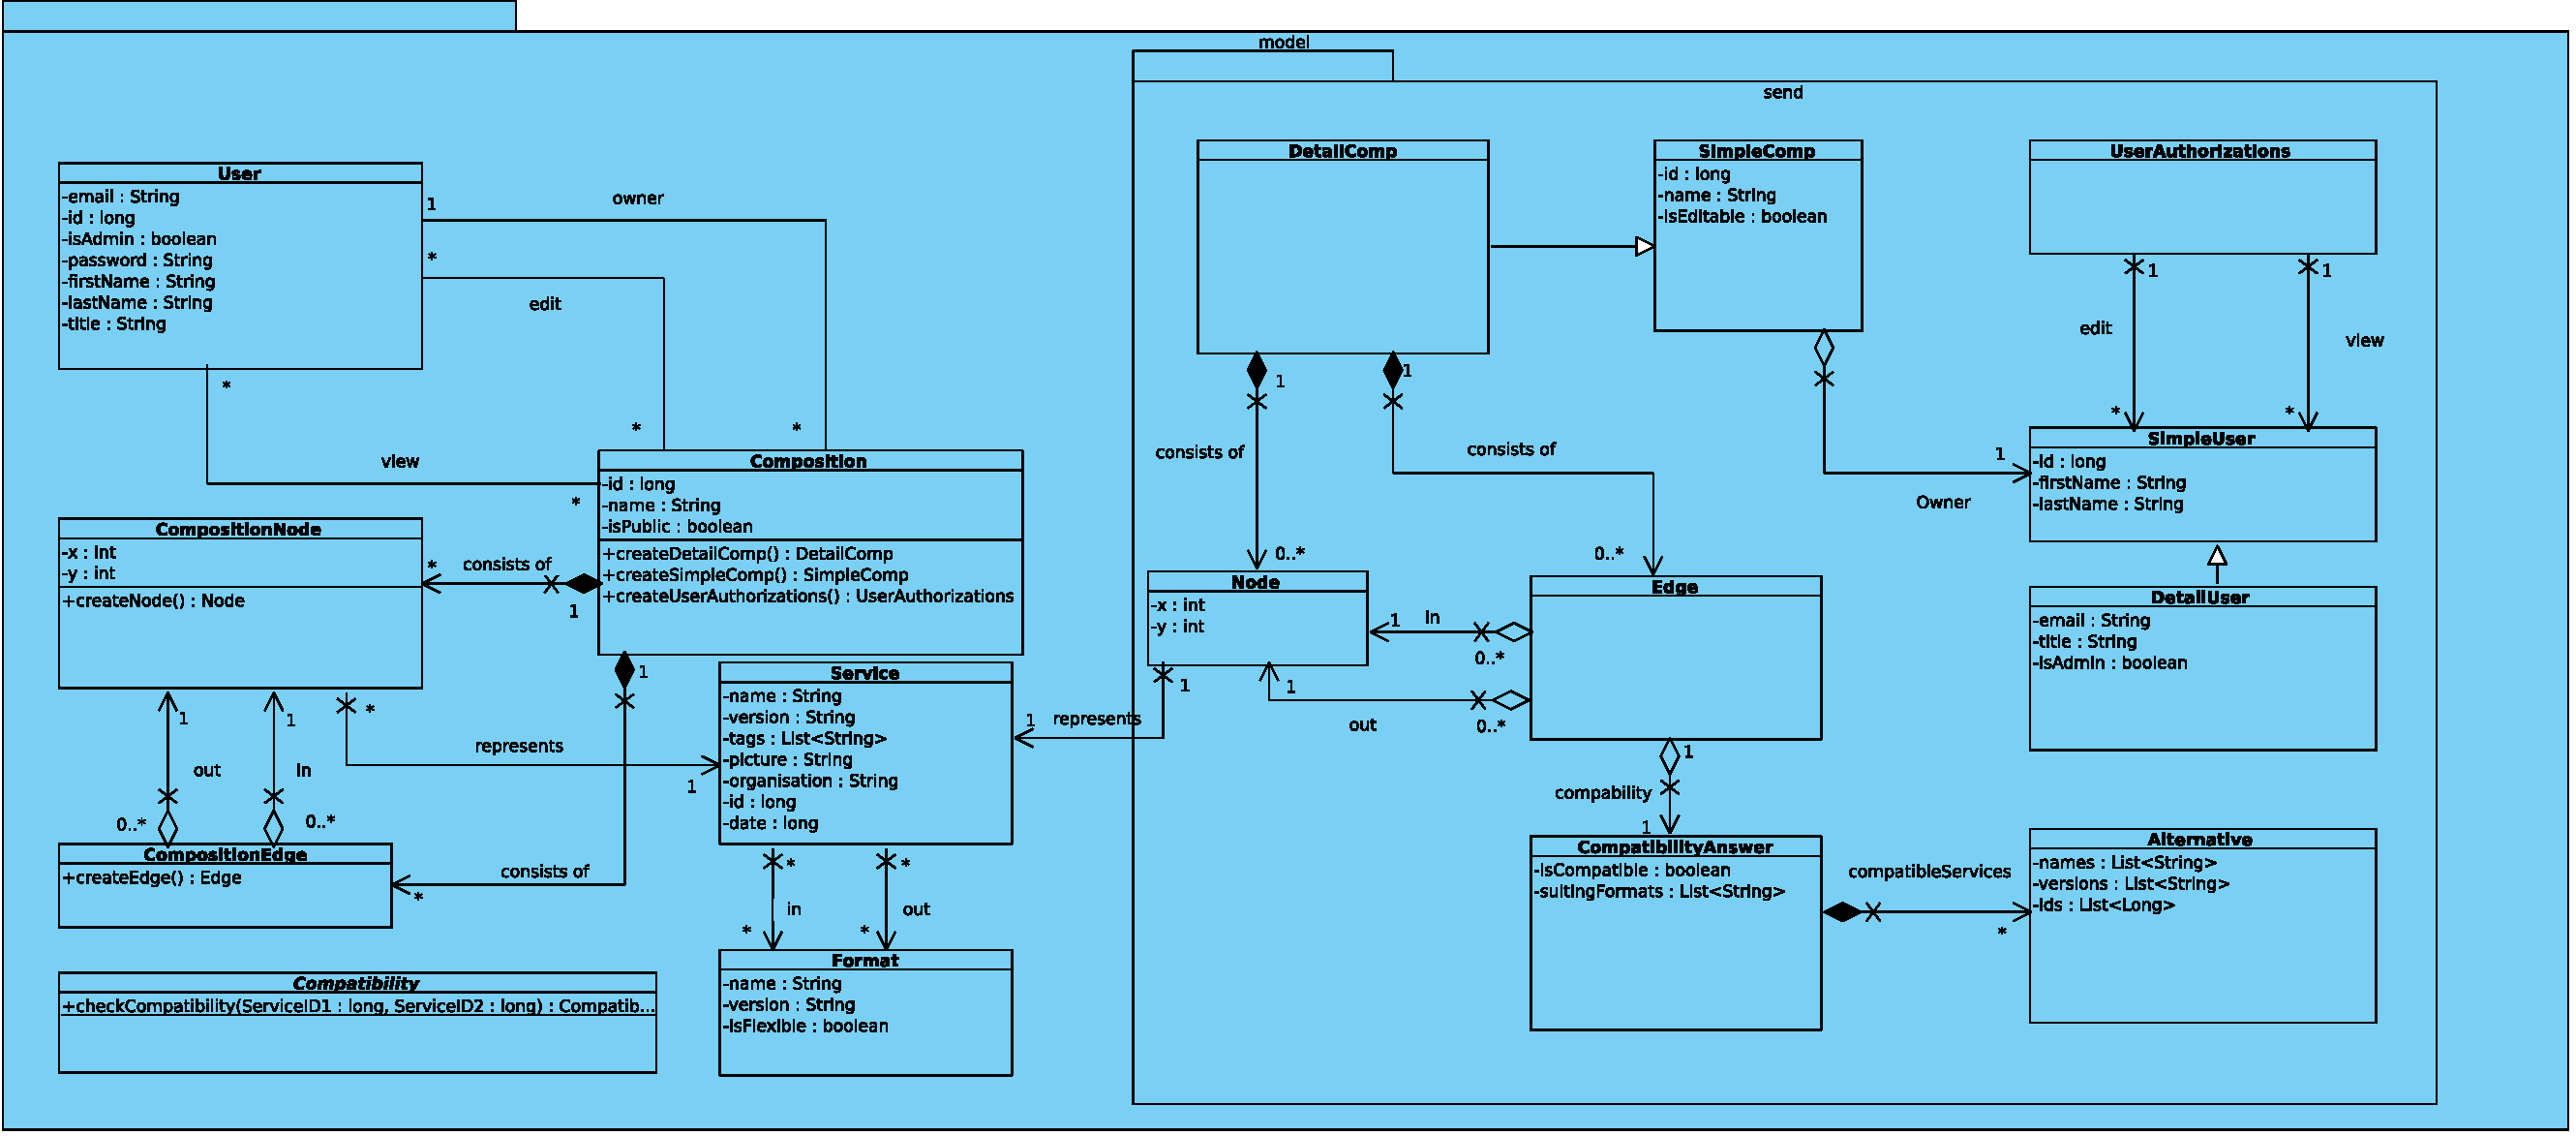
\includegraphics[width=\textwidth]{img/Diagramme/Klassen/Model}
	\caption{Klassendiagramm des Models}
	\label{fig:klassendiagramm-model}
\end{figure}

\paragraph{User}
\begin{itemize}
		\item Speicherung der Nutzerdaten, sowie einer künstlichen Datenbank-ID
		\item Eine Flag, die den Adminstatus festlegt
		\item Listen von erstellten, einsehbaren und veränderbaren Kompositionen
\end{itemize}

\paragraph{Composition}
\begin{itemize}
	\item Speicherung einer künstlichen ID
	\item Speicherung der Kompositionen als Graphen, durch Speicherung der Knoten und Kanten
	\item Speicherung des Urhebers und der Nutzenden mit Zugriffs- bzw. Bearbeitungsrechten
	\item Konvertermethode, zum Erstellen eines detaillierten, versendbaren Objektes
	\item Konvertermethode, zum Erstellen eines reduzierten Objektes
	\item Methode zum Erstellen eines UserAuthorizations-Objektes um Nutzerrechte später einzusehen
\end{itemize} 

\paragraph{CompositionNode}
\begin{itemize}
	\item Speicherung eines Dienstes, für dessen Verwendung im Kompositionsgraphen
	\item Konvertermethode, zum Erstellen eines detaillierten, versendbaren Objektes
	\item Referenz auf CompatibilityAnswer um Kompatibilität der verbundenen Dienste darzustellen
\end{itemize} 
\paragraph{CompositionEdge} 
\begin{itemize}
	\item Speicherung einer gerichteten Kompositionskante als Paar von Kompositionsknoten
	\item Konvertermethode, zum Erstellen eines detaillierten, versendbaren Objektes
\end{itemize}

\paragraph{Service}
\begin{itemize}
	\item Speicherung der Diensteigenschaften
	\item Speicherung der zum Dienst gelisteten Tags
	\item Speicherung einer künstlichen ID
	\item Speicherung je einer Liste der passenden Ein- bzw. Ausgabeformate
\end{itemize} 
\paragraph{Format}
\begin{itemize}
	\item Speicherung von Name, Version und Kompatibilitätsgrad
\end{itemize} 
\paragraph{Compatibility}
\begin{itemize}
	\item Utilklasse
	\item Methode zum bestimmen der Kompatibilität zweier Dienst
	\item Methode soll für Einzelanfragen und Kanten verwendet werden
\end{itemize} 



\paragraph{DetailComp}
\begin{itemize}
	\item Erbt von SimpleComp und speichert damit Metadaten zur Komposition (ob bearbeitbar, Name und ID)
	\item Listen der User (als SimpleUser) mit Bearbeitungs- bzw Einsichtrecht
	\item Verweis auf Autor
\end{itemize}
\paragraph{Edge}
\begin{itemize}
	\item Besteht aus einem geordneten Paar von Nodeobjekten, dem Eingang- und Ausgangsknoten.
	\item Speicherung der Kompatibilität der Dienste anhand einer CompatibilityAnswer
\end{itemize}
\paragraph{Node} 
\begin{itemize}
	\item Speicherung der Position und Verweis auf den verwendeten Service
\end{itemize}
\paragraph{SimpleComp}
\begin{itemize}
	\item Speicherung der elementarsten Daten für die Listenansicht der Komposition
\end{itemize}
\paragraph{SimpleUser}
\begin{itemize}
	\item Speicherung der elementarsten Daten (ID und Name)
\end{itemize}
\paragraph{DetailUser}
\begin{itemize}
	\item Erbt von SimpleUser
	\item Dient der Bearbeitung der User
	\item Flag um User als Administratoren zu markieren
	\item Kein Passwortvermerk
\end{itemize}
\paragraph{Alternative}
\begin{itemize}
	\item Speicherung der möglichen Konverter eventuell Konverterketten (Name, Versionsnummer, ID) um Kompatibilität zu erzeugen
\end{itemize}
\paragraph{CompatibillityAnswer}
\begin{itemize}
	\item Speicherung der Kompatibilität zwischen zwei Diensten
	\item Speicherung der effektiv kompatiblen Formate
	\item Liste von Alternativen
	\item Zum Antworten auf Einzelanfragen zur Kompatibilitätsprüfung zweier Dienste
\end{itemize}
\paragraph{UserAuthorizations}
\begin{itemize}
	\item Speicherung je einer Liste für User mit Einsichts- bzw. Bearbeitungsrecht
\end{itemize}


\begin{figure}[!h]
	\centering
	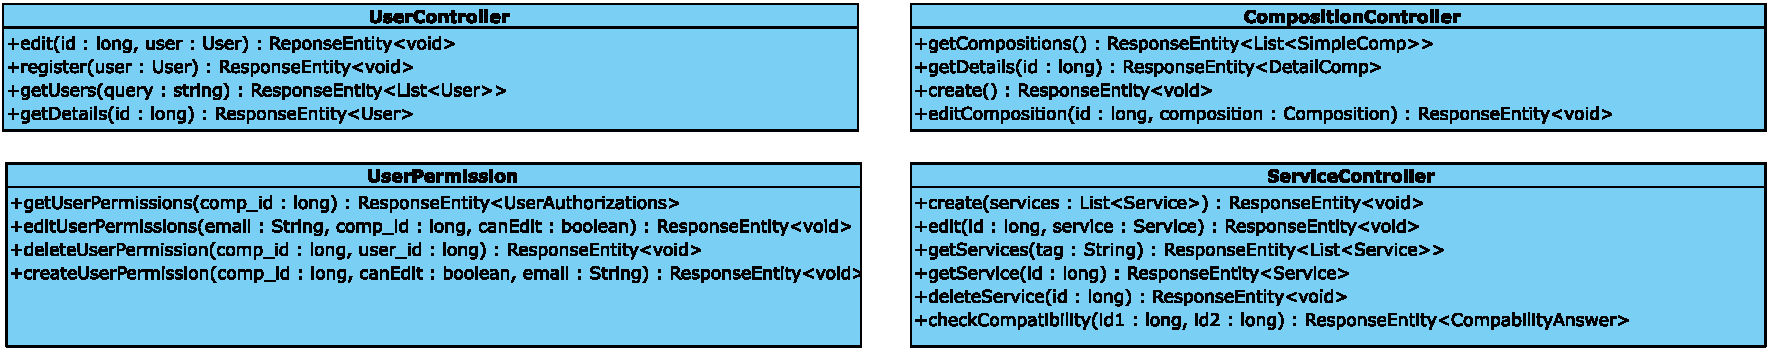
\includegraphics[width=\textwidth]{img/Diagramme/Klassen/Controller}
	\caption{Klassendiagramm des Controllers}
	\label{fig:klassendiagramm-controller}
\end{figure}


\paragraph{CompositionController}
\begin{itemize}
	\item Klasse stellt einen REST-Controller dar
	\item Verschiedene Methoden zum Erstellen, Anfragen und bearbeiten von Compositions aus der Datenbank
	\item die Authorisierung des Nutzers wird in der Behandlung der Anfragen berücksichtigt
	\item Rückgabetyp ist stets ResponseEntity, da so ein entsprechender HTTP-Code als Antwort gegeben werden kann.
\end{itemize}
\paragraph{ServiceController}
\begin{itemize}
	\item Rest-Controller, analog zu CompositionController
	\item Verwaltet den Zugriff und Bearbeitung von Servicen.
\end{itemize}
\paragraph{UserController}
\begin{itemize}
	\item REST-Controller, analog zu den anderen Klassen
	\item Erlaubt es Daten von User zu verändern
\end{itemize}
\paragraph{UserPermission}
\begin{itemize}
	\item REST-Controller
	\item Erlaubt es dem Owner einer Komposition die Zugriffsrechte auf selbige zu verändern.
\end{itemize}

\newpage
\section*{Klassendiagramm zur Android-App}

\begin{figure}[!h]
	\centering
	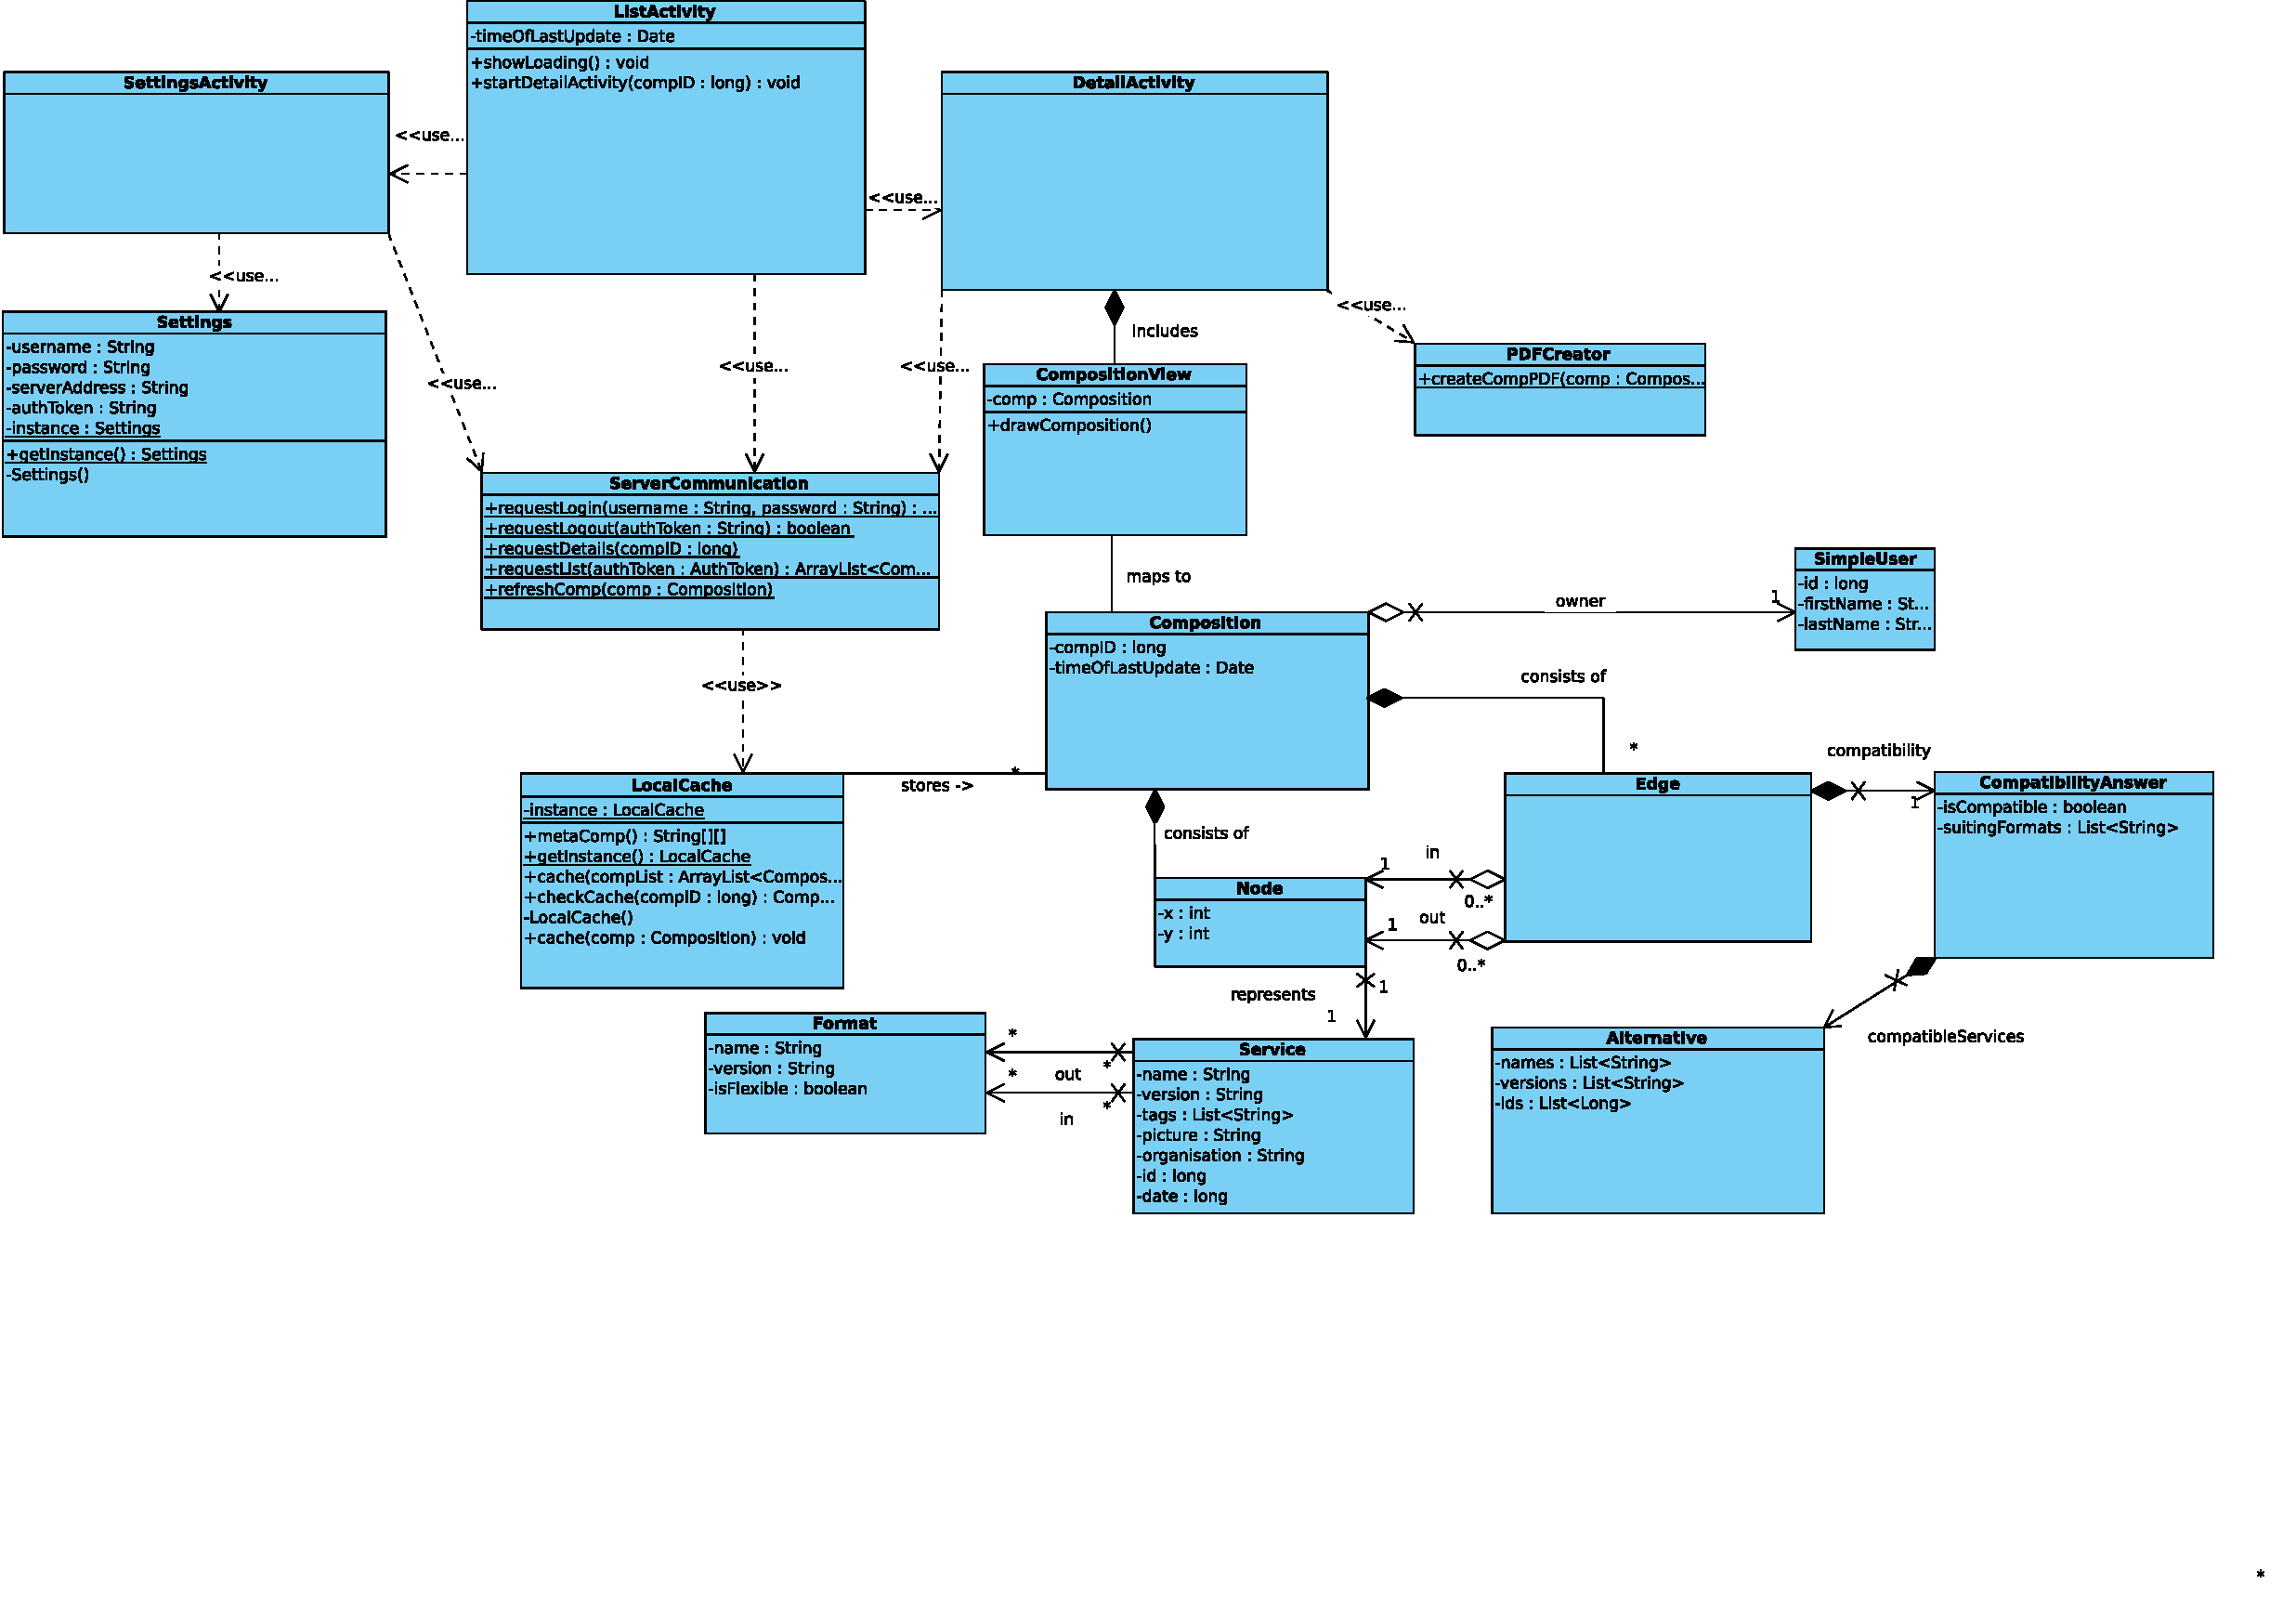
\includegraphics[width=\textwidth]{img/Diagramme/Klassen/App}
	\caption{Klassendiagramm - App}
	\label{fig:klassendiagramm-app}
\end{figure}

\paragraph{ListActivity}
\begin{itemize}
	\item MainActivity und Übersicht über sichtbare Kompositionen 
\end{itemize}
\paragraph{SettingsActivity}
\begin{itemize} 
	\item Activity zum Festlegen von Einstellungen, zum Einloggen und Festlegen der Serveradresse 
\end{itemize} 
\paragraph{DetailActivity}
\begin{itemize}
	\item Detailansicht zur grafischen Darstellung einer Komposition 
\end{itemize}
\paragraph{Settings} 
\begin{itemize}		
	\item Dient zur Kapselung der getroffenen Einstellungen 
\end{itemize}
\paragraph{CompositionView}
\begin{itemize}
	\item Eigentliche View, in der das Zeichnen einer Komposition stattfindet. 
	\item Jede DetailActivity verfügt über ein CompositionView. 
\end{itemize}
\paragraph{Composition}
\begin{itemize}
	\item Model-Abstraktion einer Komposition 
\end{itemize}
\paragraph{Node}
\begin{itemize}
	\item Interne Model-Abstraktion eines Diensts, der als Knoten in einer Komposition fungiert. 
\end{itemize}
\paragraph{Edge} 
\begin{itemize}
	\item Interne Model-Abstraktion einer Kante zwischen zwei Diensten in einer Komposition 
\end{itemize}
\paragraph{PDFCreator}
\begin{itemize}
	\item Helper-Klasse zur Generierung von PDFs, die Kompositionsbilder beinhalten. 
\end{itemize}

\paragraph{ServerCommunication}
\begin{itemize} 
	\item Anlaufpunkt für sämtliche Kommunikation mit dem Backend. 
	\item ServerCommunication übernimmt die Aufgabe, Verbindungen zum Server herzustellen, die Daten zu interpretieren und im richtigen Format weiterzugeben. 
\end{itemize}
\paragraph{LocalCache}
\begin{itemize} 
	\item Cache zur Speicherung von durch Anfragen erhaltenden Daten, damit diese nicht erneut angefragt werden müssen. 
\end{itemize}
\paragraph{Service}
\begin{itemize} 
	\item Interne Abbildung eines Diensts
	\item Kapselt sämtlich relevante Informationen eines Services
	\item Verfügt über Verweis auf In- und Out-Formate
\end{itemize}
\paragraph{Format}
\begin{itemize}	
	\item Format eines Services mit Version, Flexible-Flag und Name.
\end{itemize}
\paragraph{CompatibilityAnswer}
\begin{itemize}
	\item Kapselt die Auswertung, ob ein Dienstpaar beziehungsweise eine Kante kompatibel ist. 
	\item Gleichzeitig speichert es die passenden Formate des Dienstpaars beziehungsweise einer Kante
	\item Gibt es Alternativen, finden sich diese in einer Liste, die als Instanzvariable abgelegt ist.
\end{itemize}
\paragraph{Alternative} 
\begin{itemize}
	\item Speichert die Alternativen eines inkompatiblen Dienstpaares.
\end{itemize}

\newpage
\section*{Klassendiagramm zum Web-Frontend}

\begin{figure}[!h]
	\centering
	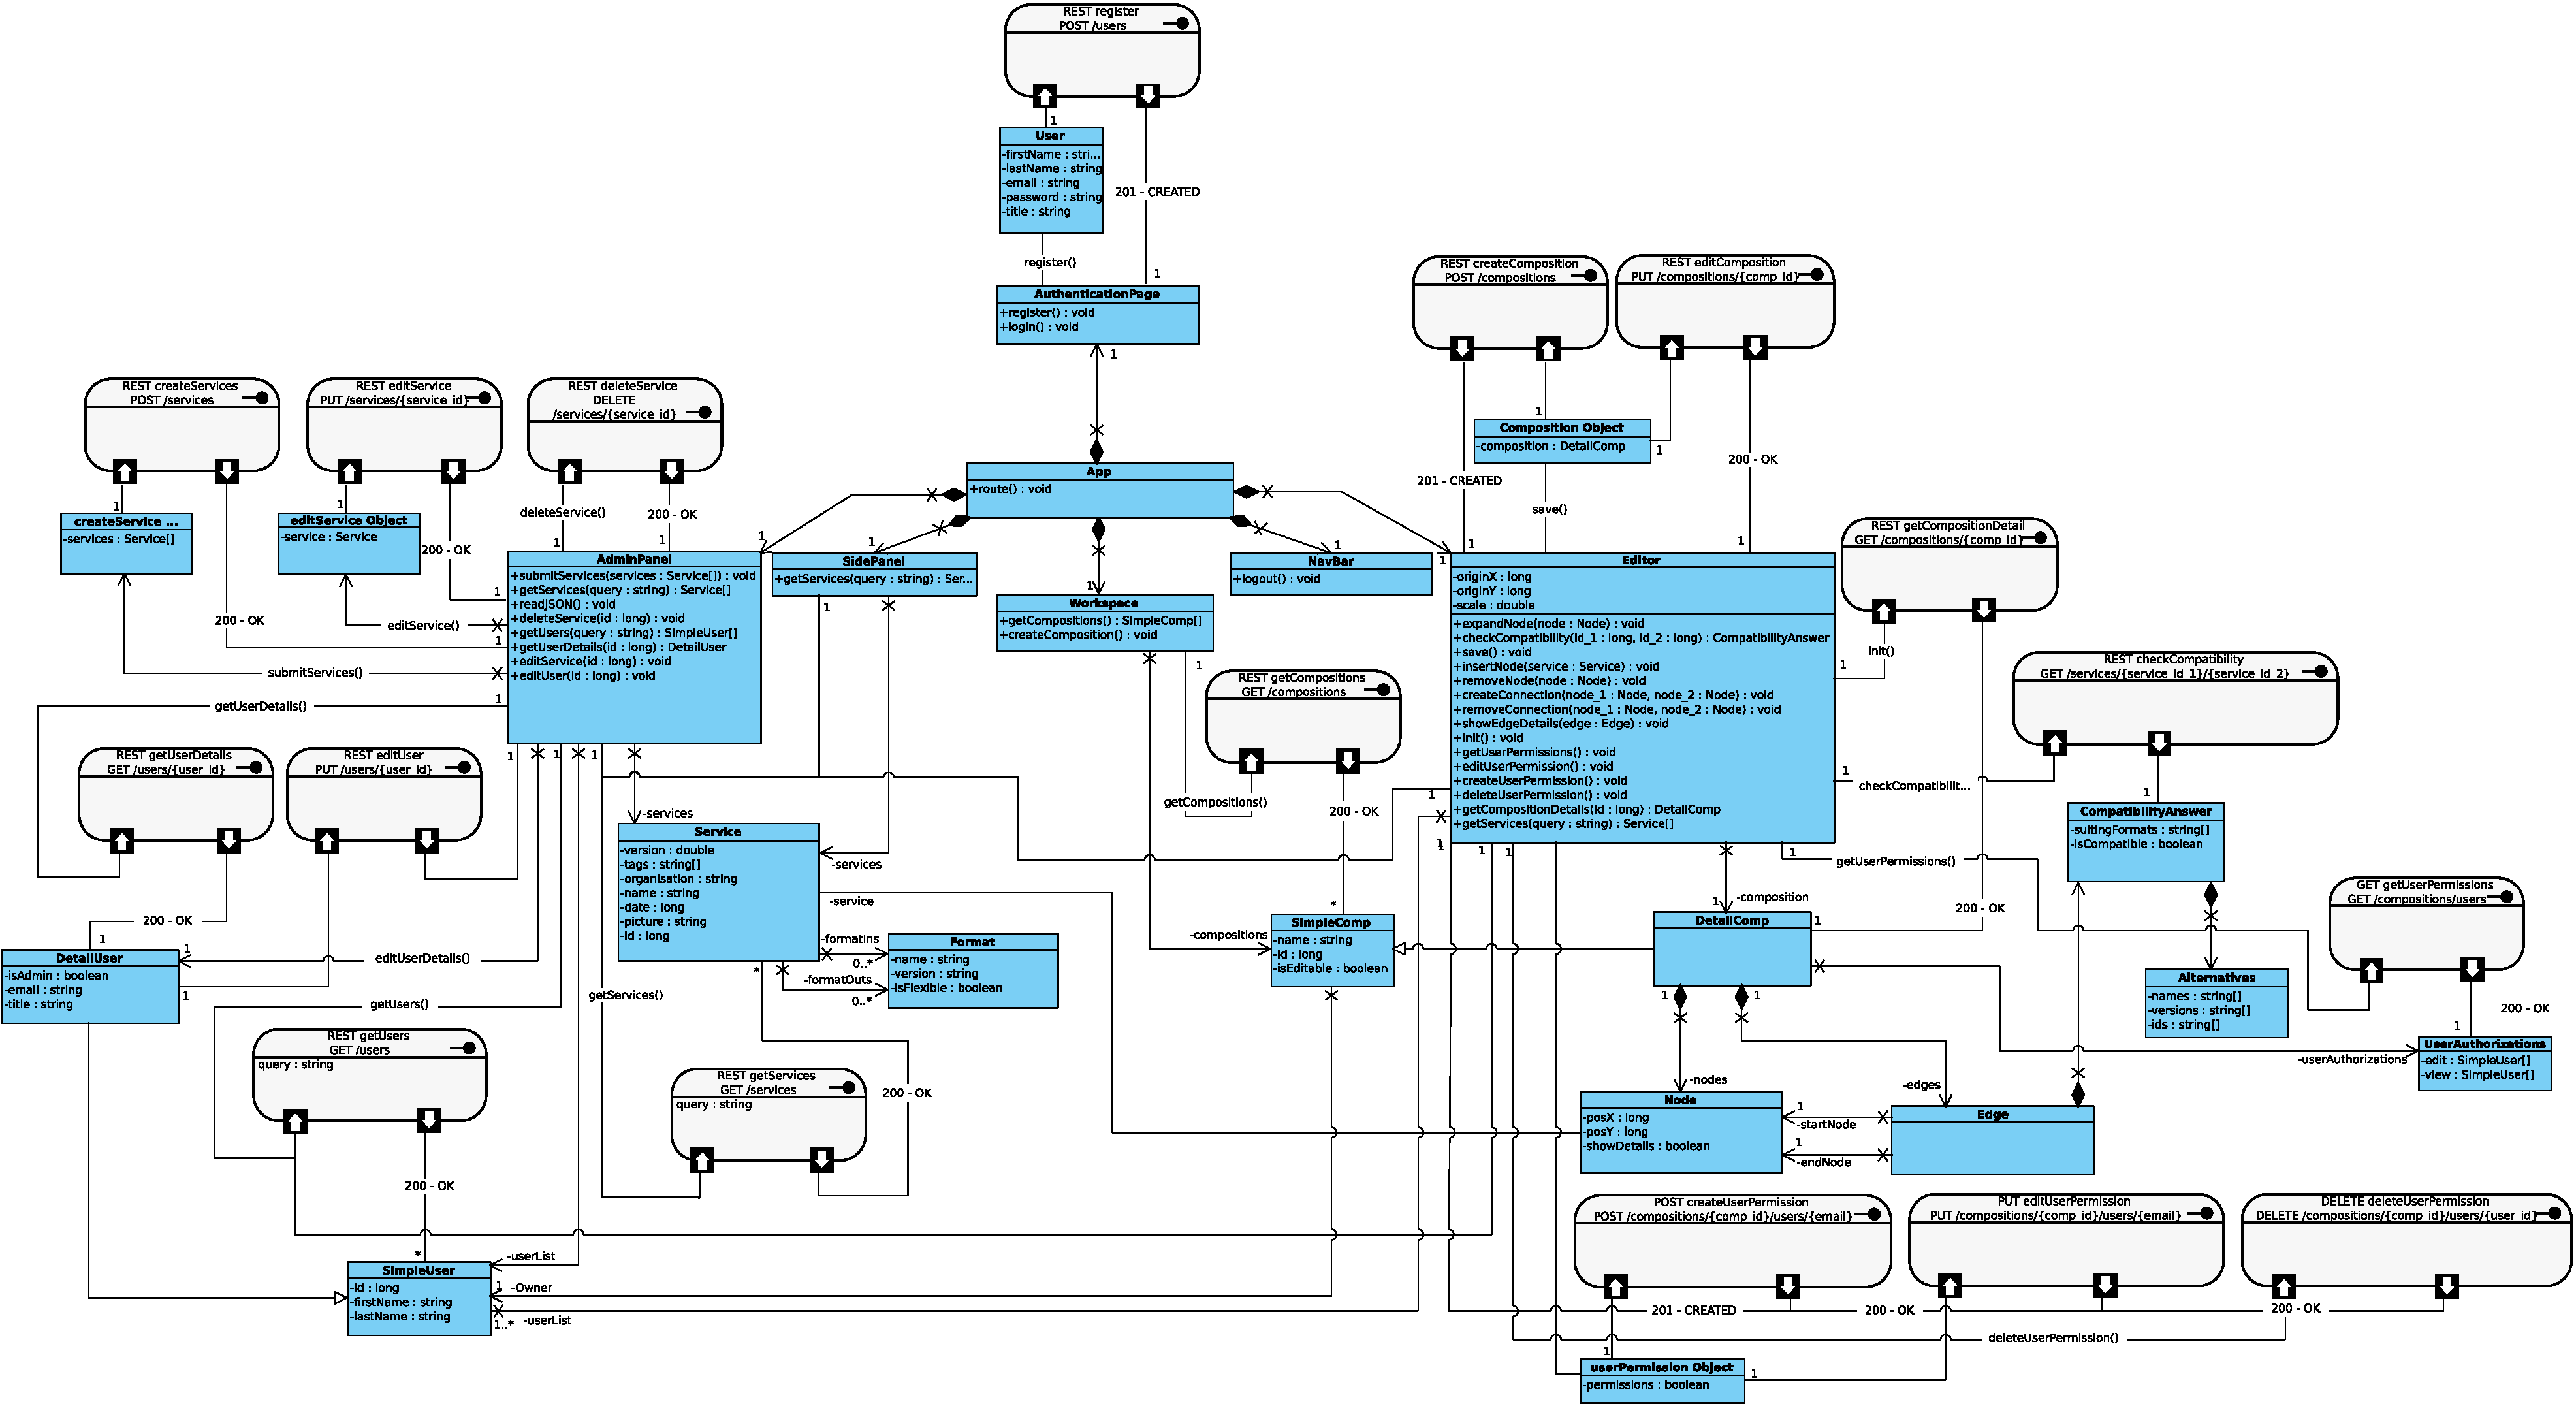
\includegraphics[width=\textwidth]{img/Diagramme/Klassen/Frontend}
	\caption{Klassendiagramm - Web}
	\label{fig:klassendiagramm-web}
\end{figure}

\paragraph{App}\mbox{}\\
Alle Anfragen, die nicht an die REST-Schnittstelle vom Server gehen, werden hierhin zurück geleitet
und dann entsprechend von hier aus geroutet.
\paragraph{AuthenticationPage}\mbox{}\\
Bietet die Möglichkeit über eine Maske sich einzuloggen oder zu registrieren.
\paragraph{AdminPanel}\mbox{}\\
Bietet die Möglichkeiten, Services zu erstellen, bearbeiten und löschen und Rechte von Nutzern zu bearbeiten. 
\paragraph{SidePanel}\mbox{}\\
Ruft Services ab, stellt sie dar und lässt die angezeigten Services mit einer Suche einschränken. 
\paragraph{Workspace}\mbox{}\\
Zeigt eine Liste von allen einsehbaren und bearbeitbaren Kompositionen. 
\paragraph{NavBar}\mbox{}\\
Stellt einige Informationen zum Login-Status dar und ermöglicht den logout.
\paragraph{Editor}\mbox{}\\
Hier wird die Detailansicht einer Komposition angezeigt mit der Möglichkeit, diese durch Hinzufügen und Entfernen von
Diensten und Kanten zu verändern, sofern die nötigen Rechte vorhanden sind. Es kann auch vom Autor der Komposition festgelegt
werden, welche Nutzer die Komposition einsehen und bearbeiten können. 
\paragraph{restlichen Klassen}\mbox{}\\
Dienen zur Modellierung der Objekte, die über die REST-Schnittstelle ausgetauscht werden. 


	\chapter{Sequenzdiagramme}\label{chp:sequenzdiagramme}
	\thispagestyle{fancy}
		Das dynamische Verhalten des Systems wird mittels Sequenzdiagrammen modelliert.
	Hier wird zunächst ein grobes geräteübergreifendes Diagramm vorgestellt.
	Die restlichen Sequenzdiagramme beziehen sich nur auf wichtige Methoden in den gekapselten Ökosystemen APP, Website und Backend. Deswegen werden Lost und Found Messages verwendet, um die Kommunikation mit dem Server darzustellen. 
	

\subsection*{Sequenzdiagramm: Öffnen der ListActivity}

\begin{figure}[h]
	\centering
%\includegraphics[width= \linewidth ]{img/SDListAct.svg}
	\missingfigure{Sequenzdiagramm}			
	\caption{Sequenzdiagramm - Öffnen der ListActivity}
	\label{fig:sequenz-a}
\end{figure}
\noindent
Dieses Sequenzdiagramm zeigt den Vorgang, der abläuft, wenn die ListActivity initial gestartet wird und mit einer Liste aus Kompositionseinträgen zu füllen ist.
Da der Nutzer noch nicht eingeloggt ist, wird eine requestList()-Anfrage ohne Token gestartet. Diese wird in einem eigenen Thread ausgeführt, damit der UI-Thread nicht blockiert. Die Methode requestList() führt einen HTTPS-Request an das Backend aus. In der Zeit, in der die ListActivity die Antwort noch nicht erhalten hat, zeigt sie mithilfe von showLoading() eine Ladeanimation an.

\section*{Sequenzdiagramme der App}
\subsection*{Sequenzdiagramm: Klicken auf Kompositionseintrag}

\begin{figure}[h]
	\centering
	%\includegraphics[width= \linewidth ]{img/SDDetail.svg}
	\missingfigure{Sequenzdiagramm}		
	\caption{Sequenzdiagramm - Klick auf Kompositionseintrag}
	\label{fig:sequenz-a}
\end{figure}

Dieses Sequenzdiagramm beginnt damit, dass der Nutzer auf ein Listenelement tippt, um die Detailansicht aufzurufen. 
Dadruch wird die Methode startDetailActivity() aufgerufen, die die Klasse ServerCommunication veranlasst, im LokalCache nach der gewünschten Komposition zu suchen.
Falls diese noch nicht im Cache ist, wird ein HTTPS-Request an den Server gesendet.
In der Antwort sind dann alle nötigen Details der Komposition enthalten.
Diese werden dann im LokalCache abgelegt und an die ListActivity zurückgegeben.
Damit wird dann ein Intent erstellt und die DetailActivity gestartet.
\\
Da LocalCache ein Singleton ist, muss zu Beginn die Instanz abgerufen werden. Wir planen die Instanz vorzudefinieren (eager instantiation), wodurch der Fall, dass die Instanz erst erzeugt werden muss, nie eintritt.
\\
Die Methode httpsRequest() wird nicht implementiert, sondern dient hier zur Abstraktion. In der Implementation wird diese Abfrage asynchron ablaufen und in einem anderen Thread laufen, so dass der UI-Thread nicht blockiert wird. 



\end{document}
